\documentclass[]{book}

%These tell TeX which packages to use.
\usepackage{array,epsfig}
\usepackage{amsmath}
\usepackage{amsfonts}
\usepackage{amssymb}
\usepackage{amsxtra}
\usepackage{amsthm}
\usepackage{mathrsfs}
\usepackage{color}
\usepackage{pgfplots}

%Here I define some theorem styles and shortcut commands for symbols I use often
\theoremstyle{definition}
\newtheorem{defn}{Definition}
\newtheorem{thm}{Theorem}
\newtheorem{cor}{Corollary}
\newtheorem*{rmk}{Remark}
\newtheorem{lem}{Lemma}
\newtheorem*{joke}{Joke}
\newtheorem{ex}{Example}
\newtheorem*{soln}{Solution}
\newtheorem{prop}{Proposition}

\newcommand{\lra}{\longrightarrow}
\newcommand{\ra}{\rightarrow}
\newcommand{\surj}{\twoheadrightarrow}
\newcommand{\graph}{\mathrm{graph}}
\newcommand{\bb}[1]{\mathbb{#1}}
\newcommand{\Z}{\bb{Z}}
\newcommand{\Q}{\bb{Q}}
\newcommand{\R}{\bb{R}}
\newcommand{\C}{\bb{C}}
\newcommand{\N}{\bb{N}}
\newcommand{\M}{\mathbf{M}}
\newcommand{\m}{\mathbf{m}}
\newcommand{\MM}{\mathscr{M}}
\newcommand{\HH}{\mathscr{H}}
\newcommand{\Om}{\Omega}
\newcommand{\Ho}{\in\HH(\Om)}
\newcommand{\bd}{\partial}
\newcommand{\del}{\partial}
\newcommand{\bardel}{\overline\partial}
\newcommand{\textdf}[1]{\textbf{\textsf{#1}}\index{#1}}
\newcommand{\img}{\mathrm{img}}
\newcommand{\ip}[2]{\left\langle{#1},{#2}\right\rangle}
\newcommand{\inter}[1]{\mathrm{int}{#1}}
\newcommand{\exter}[1]{\mathrm{ext}{#1}}
\newcommand{\cl}[1]{\mathrm{cl}{#1}}
\newcommand{\ds}{\displaystyle}
\newcommand{\vol}{\mathrm{vol}}
\newcommand{\cnt}{\mathrm{ct}}
\newcommand{\osc}{\mathrm{osc}}
\newcommand{\LL}{\mathbf{L}}
\newcommand{\UU}{\mathbf{U}}
\newcommand{\support}{\mathrm{support}}
\newcommand{\AND}{\;\wedge\;}
\newcommand{\OR}{\;\vee\;}
\newcommand{\Oset}{\varnothing}
\newcommand{\st}{\ni}
\newcommand{\wh}{\widehat}

%Pagination stuff.
\setlength{\topmargin}{-.3 in}
\setlength{\oddsidemargin}{0in}
\setlength{\evensidemargin}{0in}
\setlength{\textheight}{9.in}
\setlength{\textwidth}{6.5in}
\pagestyle{empty}



\begin{document}

\subsection*{Exo 1}
Rappel de cours:
\begin{itemize}
\item Une fonction d\'erivable est continue, par contre le r\'eciproque n'est pas vraie
\item Une fonction est d\'erivable sur un intervalle si elle est d\'erivable en tout point de cette intervalle
\item Une fonction est d\'erivable en un point $a$ si $\exists l, \lim_{x \to a}\frac{f(x)-f(a)}{x-a} = l$ ou $\exists l, \lim_{h \to 0}\frac{f(a+h)-f(a)}{h}$
\item une fonction est d\'erivable sur un intervalle donné si elle est un assemblage de fonctions connues et dérivables sur cette intervalle.
\end{itemize}

La fonction $f(x) = |x-\pi| sin(x)$ est \'egale \`a
$$f(x) = 
\left\{ 
\begin{array}{l l}
 (x-\pi) sin(x) & x \ge \pi \\
 (\pi-x) sin(x) & x < \pi \\
\end{array}
\right. 
$$

Les deux parties sont un assemblage fonctions d\'erivables sur leur intervalle. Il reste \`a d\'emontrer si la fonction est d\'erivable en $\pi$.
$$\exists l, \lim_{x \to \pi}\frac{f(x)-f(\pi)}{x-\pi} = l$$
$$ 
\left\{ 
\begin{array}{l}
 \lim_{x \to \pi^{+}}\frac{(x-\pi) sin(x) - (\pi-\pi) sin(\pi)}{x-\pi} \\
 \lim_{x \to \pi^{-}}\frac{(\pi-x) sin(x) - (\pi-\pi) sin(\pi)}{x-\pi} \\
\end{array}
\right. 
$$

$$ 
\left\{ 
\begin{array}{l}
 \lim_{x \to \pi^{+}}\frac{(x-\pi) sin(x)}{x-\pi} \\
 \lim_{x \to \pi^{-}}\frac{-(x-\pi) sin(x)}{x-\pi} \\
\end{array}
\right. 
$$

$$ 
\left\{ 
\begin{array}{l}
 \lim_{x \to \pi^{+}} sin(x) \\
 \lim_{x \to \pi^{-}} -sin(x) \\
\end{array}
\right. 
$$

La fonction sinus est impaire, $sin(-x) = -sin(x)$. Donc

$$ 
\left\{ 
\begin{array}{l}
 \lim_{x \to \pi^{+}} sin(x) \\
 \lim_{x \to \pi^{-}} sin(-x) \\
\end{array}
\right. 
$$

on a $\lim_{x \to \pi^{-}} sin(-x) = \lim_{x \to \pi^{+}} sin(x)$. La valeur $l$ existe donc la fonction $f$ est d\'erivable.\\

La proposition est Vraie.

\subsection*{Exo 2}

Soit $f(x) = e^{x}$. on a $\forall x, f'(x) = e^{x}$
$$\lim_{h \to 0}\frac{f(x_0+3h)-f(x_0+h)}{h}$$
$$\lim_{h \to 0}\frac{e^{(x_0+3h)} - e^{(x_0+h)}}{h}$$
$$\lim_{h \to 0}\frac{e^{x_0}.e^{3h} - e^{x_0}.e^{h}}{h}$$
$$\lim_{h \to 0}\frac{e^{x_0}(e^{3h}-e^{h})}{h}$$
$$e^{x_0}\lim_{h \to 0}\frac{(e^{3h}-e^{h})}{h}$$

Si $\lim_{h \to 0}\frac{f(x_0+3h)-f(x_0+h)}{h} = 2f'(x_0)$ alors on a $\lim_{h \to 0}\frac{(e^{3h}-e^{h})}{h} = e^{x_0}$. Ce qui est faux.\\

La proposition est Fausse.

\subsection*{Exo 3}


\subsection*{Exo 4}
Soit $f(x) = (x-1)^3$, le fonction est d\'erivable $f'(x)=3(x-1)^2$ et $f'(1) = 0$. Le point $1$ n'est pas un extremum de la fonction sur l'intervalle $[-2,3]$. En effet, $f(-2) = -27 < f(1) = 0$ donc $1$ n'est pas un minimum local et $f(3) = 8 > f(1) = 0$ donc $1$ n'est pas un maximum local.\\

La proposition est Fausse.\\

\begin{tikzpicture}
	\begin{axis}[
        axis lines = middle,
		xlabel=$x$,
		ylabel={$f(x) = (x-1)^3$},
		grid=major,
	]
	% use TeX as calculator:
	\addplot [
   domain=-2:3,
   samples=100,
   color=blue]
   {(x-1)^3};
	\end{axis}
\end{tikzpicture}



\subsection*{Exo 5}
Soit $f(x) = |x|$, la fonction est d\'efinie et continue en $0$ mais pas d\'erivable en $0$.
En effet, si $f(x)$ est d\'erivable en $a$ alors, $\exists l, \lim_{x \to a}\frac{f(x)-f(a)}{x-a} = l$

$$ 
\left\{ 
\begin{array}{l}
 \lim_{x \to 0^{+}} \frac{x - 0}{x-0} = 1 \\
 \lim_{x \to 0^{-}} \frac{-x - 0}{x-0} = -1 \\
\end{array}
\right. 
$$

La proposition est Fausse.

\end{document}

